\documentclass[sigconf,anonymous,review]{acmart}
\usepackage{popets}

\usepackage[american]{babel}
\usepackage[english=american]{csquotes}

\usepackage[T1]{fontenc}
% \usepackage{cite}
\usepackage{amsmath,amsfonts} %,amssymb
\usepackage{graphicx}
\usepackage{textcomp}
\usepackage{bmpsize}
\usepackage{lipsum}
% \usepackage[colorlinks=true,urlcolor=black]{hyperref}

\usepackage{balance}
\usepackage{float}
\usepackage[dvipsnames]{xcolor}
\usepackage{tabularx}
\usepackage[textsize=footnotesize, textwidth=35mm]{todonotes} % \todo and \todo[inline]
\presetkeys{todonotes}{fancyline}{}
\setlength{\marginparwidth}{15mm}
\usepackage{paralist}
\usepackage{enumitem}
\usepackage{comment}
\usepackage{wasysym} % Add this in your preamble for the circle symbols
% \usepackage{stfloats} %[!b] for bottom-page figure
\usepackage{subcaption}

\usepackage{relsize} % for \mathlarger
% Colors tuto: https://www.overleaf.com/learn/latex/Using_colors_in_LaTeX
% \defincolor: {define new color}
%   - rgb: {r, g, b}                            [0, 1]
%   - RGB: {r, g, b}                            [0, 255]
%   - hsb: {hue, saturation, brightness}        [0, 1]
%   - HSB: {hue, saturation, brightness}        [360°, 100%, 100%]
%   - cmy: {cyan, magenta, yellow}              [0, 1]
%   - cmyk: {cyan, magenta, yellow, blacK}      [0, 1]
%   - gray: {gray}                              [0, 1] (low is dark)
%   - Gray: {Gray}                              [0, 15] (low is dark)
%   - HTML: {RRGGBB}                            6 hexa-digits
%   - wave: {wavelength}                        [363, 814] (nm)
% \colorlet: (i.e. mixing colors)
%   - \colorlet{mixedColor}{blue!10!red}        % 10% blue mixed with 90% red

\definecolor{unHighlight}{gray}{0.60}

\newcommand{\bigO}[1]{$\mathcal{O}(#1)$}

\newcommand{\mathtext}[1]{\text{\scriptsize #1}}
% \newcommand{\indexsize}{\footnotesize}
% \renewcommand{\index}[1]{\mathtext{\indexsize {#1}}}
\renewcommand{\index}[1]{\mathtext{{#1}}}
\newcommand{\inmath}[1]{\relax\ifmmode #1 \else $#1$\fi}

\newcommand{\G}[1]{\inmath{G_\index{#1}}}
\newcommand{\N}[1]{\inmath{N_\index{#1}}}
\newcommand{\sk}[1]{\inmath{k_\index{#1}}}
\newcommand{\PK}[1]{\inmath{K_\index{#1}}}
\newcommand{\s}[1]{\inmath{s_\index{#1}}}
\renewcommand{\S}[1]{\inmath{S_\index{#1}}}

\newcommand{\sG}[2] {\relax
    \ifmmode \s{#1}\G{#2} 
    \else $\s{#1}\textcolor{unHighlight}{\G{#2}}$ 
\fi}
\newcommand{\B}[2]{\relax
    \ifmmode \mathlarger{\beta_\index{#1#2}} 
    \else $\mathlarger{\beta_\index{#1\textcolor{unHighlight}{#2}}}$ 
\fi}
\newcommand{\BB}[2]{\relax
    \ifmmode \mathlarger{\beta^\prime_\index{#1#2}} 
    \else $\mathlarger{\beta^\prime_\index{#1\textcolor{unHighlight}{#2}}}$ 
\fi}
\newcommand{\A}[1]{\inmath{\mathlarger{\mathlarger{\alpha_\index{#1}}}}}
\newcommand{\C}[1]{\inmath{\mathlarger{\mathlarger{\gamma_{\index{#1}}}}}}
\newcommand{\Cred}[1]{\inmath{\mathlarger{\mathlarger{\sigma_{\index{#1}}}}}}
\newcommand{\D}{\inmath{\mathlarger{\mathlarger{\mathrm{\Delta}}}}}

\newcommand{\hash}[1]{\inmath{\mathsf{hash}(#1)}}
\newcommand{\sHashed}[1]{\inmath{\sigma_\index{#1}}}
\newcommand{\hashIt}[2]{\inmath{\mathsf{h}^{(#2)}(#1)}}
\newcommand{\Map}[1]{\inmath{\mathsf{Encode}(#1)}}
\newcommand{\InverseMap}[1]{\inmath{\mathsf{Decode}(#1)}}
\newcommand{\InverseMapNoParenthesis}{\inmath{\mathsf{Decode}}}

\newlength{\y}
\newcommand{\width}{9mm}
\newcommand{\height}{5.4mm}

\newcommand{\vgap}{
    \addtolength{\y}{-\height}
    \addtolength{\y}{-1mm}
}
\newcommand{\vGap}{
    \addtolength{\y}{-\height}
    \addtolength{\y}{-3mm}
}
% \newcommand{\hmac}{Eq. \ref{eq:integrity}}
% \newcommand{\hmac}{\footnotesize $\sum$}

% Define TikZ styles
\usepackage{tikz}
\usepackage{tikzpeople}
\usetikzlibrary{shapes.geometric, positioning, calc, patterns, patterns.meta, backgrounds, fit, decorations.pathreplacing}

\tikzset{    
    % shape
    ovale/.style={ellipse, draw, ultra thin, minimum width = #1*\width, minimum height = \height, inner sep = 0pt, anchor = west},
    blockspace/.style={ultra thin, minimum width = #1*\width, minimum height = \height, inner sep = 0pt, anchor = west},
    block/.style={draw, blockspace = #1},
    inblock/.style={block = #1, densely dotted}, % dash pattern=on 1pt off 1pt, 
    zero_pad/.style={block = #1, fill = unHighlight, fill opacity=0.3},
    HMAC/.style={draw, ellipse, minimum width = \width, minimum height = \height, inner sep = 0pt, anchor = center},
    eq/.style={draw, circle, inner sep=1pt, fill opacity=0.2, fill=orange, text opacity=1, text=black, font=\normalsize}, %font=\bfseries\large
    arrow/.style={->, shorten <= 1pt, shorten >= 2pt},
    fleche/.style={-Latex, shorten <= 2pt, shorten >= 3pt},
    line/.style={shorten <= 1pt, shorten >= 1pt},
    dotline/.style={dotted},
    between/.style args={#1 and #2}{at = ($(#1)!0.5!(#2)$)}
}

% Put tikz node in caption
\newcommand\eq[1][black]{ % Do not know why we need [black] to works and \eq instead of {\eq}
    \hspace{-2mm}
    \tikz[baseline=(char.base)]{
        \node [eq] (char) {#1};

    }
    \hspace{-2mm}
}

\newcommand{\blindsign}[1]{ \mathord{\scalebox{1.4}{$\blind{\SIGMA}$}}_{#1} }

\newcommand{\cred}[1]{ \mathord{\scalebox{1.4}{$C$}}_{#1} }


\newcommand{\blind}[1]{\widetilde{#1}}


% \renewcommand{\paragraph}[1]{\medskip\noindent{\textbf{#1.}}}


\newlength{\greekcapheight}

\newcommand{\CapGreek}[1]{%
  \mathord{\mathpalette\CapGreekAux{#1}}%
}

\newcommand{\CapGreekAux}[2]{%
  \begingroup
  \mathsurround=0pt\relax
  \settoheight{\greekcapheight}{$#1 N$}%
  \resizebox{7pt}{\greekcapheight}{$#1#2$}%
  \endgroup
}

\newcommand{\ALPHA}{\CapGreek{\alpha}}
\newcommand{\BETA}{\CapGreek{\beta}}
\newcommand{\GAMMA}{\CapGreek{\gamma}}
\newcommand{\ETA}{\CapGreek{\eta}}
\newcommand{\ZETA}{\CapGreek{\zeta}}
% \newcommand{\NU}{\CapGreek{\nu}}
\newcommand{\KAPPA}{\CapGreek{\kappa}}
\newcommand{\PHI}{\CapGreek{\phi}}
\newcommand{\PSI}{\CapGreek{\psi}}
% \newcommand{\THETA}{\CapGreek{\theta}}
\newcommand{\XI}{\CapGreek{\xi}}
\newcommand{\SIGMA}{\CapGreek{\sigma}}
\newcommand{\RHO}{\CapGreek{\rho}}
% \newcommand{\UPSILON}{\CapGreek{\upsilon}}

\usepackage{booktabs} % \toprule, \midrule, \bottomrule
\usepackage{tablefootnote}

% \usepackage{algorithm}
% \usepackage{algpseudocode}


% % Conditional Text
% \def\isabridged{1}   % Uncomment if typesetting abridged version

% % Define and set conditionals for alternate versions
% \newif\ifabridged
% \newif\ifnotabridged

% \ifdefined\isabridged
% \abridgedtrue
% \fi

% \ifabridged\notabridgedfalse
% \else\notabridgedtrue
% \fi

% Copyright
\setcopyright{popets}
\copyrightyear{YYYY}

% Issue info
\acmYear{YYYY}
\acmVolume{YYYY}
\acmNumber{X}
\acmDOI{XXXXXXX.XXXXXXX}
\acmISBN{}
\acmConference{Proceedings on Privacy Enhancing Technologies}
\settopmatter{printacmref=false,printccs=false,printfolios=true}

\begin{document}

% The "title" command has an optional parameter, allowing the author to define a
% "short title" to be used in page headers.
\title[The Name of the Title Is Hope]{The Name of the Title Is Hope: This is the Longer Version of the Given Title}

% The "author" command and its associated commands are used to define the
% authors and their affiliations.
\author{Aurelien Chassagne}
\orcid{0009-0008-7207-868X}
\affiliation{%
  \institution{Universit\'e libre de Bruxelles}
  \city{Bruxelles}
  \country{Belgique}}
\email{aurelien.chassagne@ulb.be}

\author{Iness Ben Guirat}
\orcid{0000-0002-8766-594X}
\affiliation{%
  \institution{Universit\'e libre de Bruxelles}
  \city{Bruxelles}
  \country{Belgique}}
% \email{@ulb.be}

\author{Jan Tobias Muhlberg}
\orcid{0000-0001-5035-0576}
\affiliation{%
  \institution{Universit\'e libre de Bruxelles}
  \city{Bruxelles}
  \country{Belgique}}
% \email{@ulb.be}

\author{Jean-Michel Dricot}
\orcid{0000-0002-8539-9940}
\affiliation{%
  \institution{Universit\'e libre de Bruxelles}
  \city{Bruxelles}
  \country{Belgique}}
% \email{@ulb.be}



% By default, the full list of authors will be used in the page headers. Often,
% this list is too long, and will overlap other information printed in the page
% headers. This command allows the author to define a more concise list of
% authors' names for this purpose.
\renewcommand{\shortauthors}{Chassagne et al.}

\begin{abstract}
  Mixnets provide strong communication anonymity by hiding the relationship between senders and receivers. 
  However, large-scale deployment introduces new operational challenges, as network operators may need to enforce policies on reachable destinations, for example to support service authorization, resource management, or operational agreements. 
  Existing approaches perform destination verification at the exit gateway, where the final destination is available, but this occurs only after the traffic has already consumed the resources of the mixnet.
  %
  This paper introduces an extension of the Sphinx packet format enabling privacy-preserving destination policy enforcement. 
  Our approach integrates destination-bound credentials into the packet format, allowing a verifier to check the validity of 
  an authority-issued credential and its binding to the encrypted final destination, without revealing the destination itself. 
  This enables early rejection of unauthorized traffic while preserving destination privacy.
  %
  Our work provides a mechanism to combine destination-based policy enforcement with the anonymity properties of mixnets, avoiding the need to reveal destinations for authorization purposes.
\end{abstract}

% Keywords. The author(s) should pick words that accurately describe the work
% being presented. Separate the keywords with commas.
\keywords{Sphinx, Anonymous Credentials, Mixnet, Decentralized networks}

\maketitle

% CHECK LIST
% - The \textbf{first page must clearly state how the work is relevant to real-world privacy applications}.
% - Remove references to your institution, for example in survey materials or in git repositories. -> anonymous github
% - Use care in referring to related work, particularly your own. 
%    Do not omit references to provide anonymity, as this leaves the reviewer unable to grasp the context. 
%    Instead, reference your past work in the third person, just as you would any other piece of related work by another author.
% - manipulate other document properties (e.g., page layout, spacing, use the \textbf{\\vspace} command, fonts, figures and tables, headings), 
%    remove the copyright block (CC-BY-4.0 text, including image) on the first page, etc., in an attempt to gain an unfair advantage \textbf{will be desk-rejected}.
% - Your work should use standard \LaTeX\ sectioning commands: \verb|section|, \verb|subsection|, \verb|subsubsection|, and \verb|paragraph|. They should be numbered; do not remove the numbering from the commands.
%
% [TABLE] Table captions are placed {\itshape above} the table.
% - To set a wider table, which takes up the whole width of the page's live area, use the environment \textbf{table*}
% - Always use \textbf{midrule} to separate table header rows from data rows, and use it only for this purpose.  This enables assistive technologies to recognise table headers and support their users in navigating tables more easily.
%
% [EQUATION] in three distinct styles: inline, numbered or non-numbered display.  
% - An inline equation is produced by the \textbf{math} environment. 
% - A numbered display equation is produced by the \textbf{equation} environment. 
% - An unnumbered display equation is produced by the \textbf{displaymath} environment.
% \begin{math}
%   \lim_{n\rightarrow \infty}x=0
% \end{math},
%
% [FIGURE]
% - Figure captions are placed {\itshape below} the figure.
% - If your figure contains third-party material, you must clearly identify it as such, as shown in the example below.
% \begin{figure}[ht]
%   \centering
%   \includegraphics[width=\linewidth]{sample-franklin}
%   \caption{1907 Franklin Model D roadster. Photograph by Harris \& Ewing, Inc.
%     [Public domain], via Wikimedia Commons. (\url{https://goo.gl/VLCRBB}).}
%     \Description{A woman and a girl in white dresses sit in an open car.}
% \end{figure}
% - \textbf{Every figure should also have a figure \textbf{description} unless it is purely
% decorative. These descriptions convey what's in the image to someone who cannot
% see it. They are also used by search engine crawlers for indexing images, and
% when images cannot be loaded.} -> \url{https://authors.acm.org/proceedings/production-information/describing-figures}



% This is the end of the main body of the paper. Note the page limit of 12
% typeset pages for a normal submission, 13 pages for a revision.
% Acknowledgements, Ethical Considerations, Open Science, AI Use, References,
% and the Appendix are all outside of the main body.

\newcommand{\artifact}[0]{\url{https://github.com/}}

\nocite{sphinx}
\section{Introduction}

Mixnets is a type of anonymous communication networks that provides privacy for users on the network layer against strong adversaries. 
They achieve this via two main mechanisms: (i) delaying the messages inside the servers, also called mixnodes, such that different messages are mixed together in order to prevent a network adversary from correlating the inputs with the outputs based on timing and (ii) providing cryptographic guarantees through a packet format such as Sphinx~\cite{sphinx}, which enables secure and compact packet processing by ensuring fixed packet sizes and hiding the full routing information to achieve unlinkability. Several mixned-based systems have been proposed in the literature and many have been deployed~\cite{chaum-mix,piotrowska2017loopix,nym,danezis2003mixminion, van2015vuvuzela,lazar2018karaoke, cottrell1995mixmaster,chaum2016cmix, kwon2020xrd}. Nym is the only mixnet-based system to have recently achieved adoption at the scale of thousands of daily messages~\cite{nym}

Deploying mixnets at large scale is complex and raises several challenges, such as choosing the optimal parameters of the network~\cite{benguirat2022mixnet}, enhancing performance while keeping anonymity~\cite{das2018anonymity, ben2024blending} as well as more operational challenges such as the reputation of the nodes and managing exit policies~\cite{oram2001peer,diaz2007accountable, naylor2014balancing,mirkovic2008building, backes2014backref, xu2012accountable}.
In this paper we address the challenge of preventing abuse of exit nodes, an issue that has been discussed since the early work of anonymous communication networks. As noted by Danezis et al, ‘exit abuse is a serious barrier to wide-scale remailer deployment’~\cite{danezis2003mixminion}.

The main motivation of exit policies in Anonymous Communication Networks is to prevent network abuse, and protect the mixnodes operators from the legal risks.
Additionally, a mixnet system may need to offer a subscription-based access where users pay for the ability to anonymously communicate with a set of authorized destinations. This has been proposed by Nym whitepaper but not yet implemented~\cite{nym}. 
To the best of our knowledge all existing anonymous communication network perform verification at the exit gateway, once the final destination information is available. Since intermediate mixnodes do not learn the final destination during packet processing, they cannot verify whether the destination satisfies the network's policies.

However, this postpones policy enforcement until the traffic has already traversed the mixnet and consumed bandwidth and relay resources.


The key challenge is therefore to enable early rejection of unauthorized traffic without requiring intermediate nodes to learn the destination they are forwarding toward. Such a model requires a mechanism to verify that traffic is directed toward an authorized destination without revealing it.





This work addresses this by extending the Sphinx packet format with a privacy-preserving credential that is cryptographically bound to the encrypted destination. 
Our construction relies on a threshold multi-authority model, where authorities hold shares of a distributed signing key, 
and a client combines partial credentials from a sufficient subset of authorities without reconstructing the global secret key. 
The credential is then bound to the encrypted destination contained inside the Sphinx header and re-randomized for each packet. 
A mixnode can consequently verify that a packet carries a valid authorization for its encrypted destination without learning either the destination or the client's identity. 
The credential is updated as the packet traverses the mixnet, to be checked at any intermediate hops and prevent linkability.

The goal is not to introduce destination surveillance, but to enable privacy-preserving guarantees that communications are directed toward authorized endpoints. 
Such a mechanism provides a middle ground between unrestricted anonymous transport and destination disclosure for policy enforcement.
\newline Our contributions are summarized as follows:
\todo{phrase contributions}

% \medskip
% \noindent In summary, our main contributions are as follows:
% \begin{itemize}[topsep=1pt, itemsep=1pt]
% 	%
% 	\item Anonymous Credential design for \emph{DSphinx} (an adaptation of the Sphinx packet format)
% 	%
% 	\item We release a Python benchmark\footnote{\artifact} for measuring latency and computational overhead.
% 	%
% 	\item Security ?
% 	%
% 	\item Extra features ?
% \end{itemize}

%This paper is organized as follows... 

\section{Background and Related Work}\label{sec:related}

\subsection{Anonymous Communication Networks}

Since Chaum's seminal work on untraceable communication in 1981~\cite{chaum-mix}, mixnets have been extensively studied as a mechanism for anonymous communication~\cite{piotrowska2017loopix, van2015vuvuzela, kwon2020xrd, lazar2018karaoke, cottrell1995mixmaster, alexopoulos2017MCMIX, chaum2016cmix, chaum-mix, danezis2003mixminion}.
A mixnet is a network of servers, known as \emph{mixnodes}, that forward, delay, and shuffle messages to prevent adversaries from correlating input and output traffic. 
Each packet traverses a sequence of mixnodes before reaching its final destination, as shown in Figure~\ref{fig:mixnet}. By combining traffic mixing with layered cryptographic encryption, mixnets can provide strong communication anonymity even against powerful traffic-analysis adversaries. Messages are divided into fixed-size packets and routing information is encrypted in multiple layers, ensuring that each mixnode learns only its immediate predecessor and successor. A cryptographic packet format is therefore an essential component of a mixnet, as it protects routing information and prevents packets from being tampered or linked across hops. 
Modern mixnet designs build on these principles rely on the Sphinx packet format~\cite{sphinx}.

\begin{figure}%[t]
	\hspace{-9mm}
	\resizebox{1.085\linewidth}{!}{
\newcommand{\figonetextcol}[0]{\color{black}}

\tikzset{  
    innerLink/.style={-, densely dotted, shorten <= 1pt, shorten >= 2pt},  
    outerLink/.style={->, shorten <= 2pt, shorten >= 4pt, >=Latex},
    packet/.style={circle, inner sep=0.2pt, fill=#1},
    A/.style={packet=\colorA!40, font={#1}},
    B/.style={packet=\colorB!50, font={#1}},
    A1/.style={A=1}, A2/.style={A=2}, A3/.style={A=3}, A4/.style={A=4}, A5/.style={A=5}, A6/.style={A=6}, A7/.style={A=7}, A8/.style={A=8}, A9/.style={A=9},
    B1/.style={B=1}, B2/.style={B=2}, B3/.style={B=3}, B4/.style={B=4}, B5/.style={B=5}, B6/.style={B=6}, B7/.style={B=7}, B8/.style={B=8}, B9/.style={B=9},
}

\newcommand{\countitems}[1]{%
  \def\size{0}%
  \foreach \x in {#1} {%
    \pgfmathparse{\size+1}%
    \global\let\size=\pgfmathresult%
  }%
}

\newcommand{\outerLink}[3]{
  % size (nbr of packets)
  \countitems{#3} 
  % If odd nbr of packet, slight shift to not have a packet on an intersection
  \pgfmathparse{mod(\size,2)==1 ? \size-0.5 : \size}%
  \xdef\size{\pgfmathresult}%

  % define line
  \coordinate (start) at (#1.east);
  \coordinate (stop) at (#2.west);
  \draw[outerLink] (start) -- (stop);
  % put packet on the line
  \foreach \packet [count=\i from 1] in {#3} {
    \pgfmathsetmacro{\t}{1 - \i/(\size+1)}%
    \path let
      \p1 = (start),
      \p2 = (stop),
      \p3 = ($(\p1)!\t!(\p2)$)
    in
      node[\packet] at (\p3) {};
  }
}


\newcommand{\mixnode}[2]{%
  \countitems{#1}%

  \begin{tikzpicture}
    \def\d{0.8}
    \draw[thick] (0,0) circle (\d);

    % Connect according to mapping
    \pgfmathsetmacro{\xoffset}{(1.14*\d - \size/10)*\d}
    \foreach \r [count=\l from 1] in {#1} {
      \pgfmathsetmacro{\yposL}{\d - \l/(\size+1)*2*\d}
      \coordinate (left\l) at (-\xoffset, \yposL);
      \pgfmathsetmacro{\yposR}{\d - \r/(\size+1)*2*\d}
      \coordinate (right\l) at (\xoffset, \yposR);
    }
    % Draw dots
    \foreach \packet [count=\i from 1] in {#2} {
      \draw[innerLink] (left\i) -- (right\i);
      \node[\packet] at (left\i) {};
      \node[\packet] at (right\i) {};
    }
  \end{tikzpicture}
}

\newcommand{\client}[1]{
  \begin{tikzpicture}[scale=0.4]
    % Monitor screen
    \draw[fill=#1!20, draw=black, rounded corners=4pt] (0,0) rectangle (4,2.5);
    % Inner bezel
    \draw[fill=white, draw=none, rounded corners=3pt] (0.2,0.2) rectangle (3.8,2.3);
    % Stand
    \draw[fill=#1!40, draw=black] (1.75,-0.7) rectangle (2.25,0);
    % Base
    \draw[fill=#1!40, draw=black, rounded corners=2pt] (0.8,-1) rectangle (3.2,-0.7);
  \end{tikzpicture}
}

\newcommand{\server}[1]{
  \begin{tikzpicture}[scale=0.7]
    \foreach \y in {0, -0.6, -1.2} {
        \draw[fill=#1!20] (0,\y) rectangle (2,\y-0.5); % rectangle
        \draw (0.2,\y-0.25) circle (0.05); % power/status LED
    }
  \end{tikzpicture}
}

\newcommand{\colorA}{blue}
\newcommand{\colorB}{orange}

\newcommand{\clientA}{\client{\colorA}}
\newcommand{\clientB}{\client{\colorB}}
\newcommand{\serverA}{\server{\colorA}}
\newcommand{\serverB}{\server{\colorB}}


\begin{tikzpicture}
  \def\dx{4}
  \def\dy{-1}

  % GENERAL ARCHITECTURE (define nodes)
  \node (clientA) at (0,-\dy) {\clientA};
  \node (clientB) at (0,\dy) {\clientB};

  \node (serverA) at (4*\dx,-\dy) {\serverA};
  \node (serverB) at (4*\dx,\dy) {\serverB};

  % PACKETS - links and shuffles (python generated)
\node (mix11) at (1*\dx,-\dy) {\mixnode{3,1,2}{A2,A1,B3}};
\node (mix12) at (1*\dx, \dy) {\mixnode{3,2,1}{B2,B1,A3}};
\node (mix21) at (2*\dx,-\dy) {\mixnode{3,1,2}{A3,A2,B3}};
\node (mix22) at (2*\dx, \dy) {\mixnode{2,3,1}{B2,B1,A1}};
\node (mix31) at (3*\dx,-\dy) {\mixnode{3,1,4,2}{B2,A2,A1,B3}};
\node (mix32) at (3*\dx, \dy) {\mixnode{2,1}{A3,B1}};

\outerLink{clientA}{mix11}{A1,A2};
\outerLink{clientA}{mix12}{A3};
\outerLink{clientB}{mix11}{B3};
\outerLink{clientB}{mix12}{B1,B2};

\outerLink{mix11}{mix21}{A2,B3};
\outerLink{mix11}{mix22}{A1};
\outerLink{mix12}{mix21}{A3};
\outerLink{mix12}{mix22}{B2,B1};

\outerLink{mix21}{mix31}{A2,B3};
\outerLink{mix21}{mix32}{A3};
\outerLink{mix22}{mix31}{B2,A1};
\outerLink{mix22}{mix32}{B1};

\outerLink{mix31}{serverA}{A2,A1};
\outerLink{mix31}{serverB}{B2,B3};
\outerLink{mix32}{serverA}{A3};
\outerLink{mix32}{serverB}{B1};

  % ANNOTATIONS
  \node at (0*\dx, -2.2*\dy) {\figonetextcol Clients};
  \draw[loosely dotted, fill=gray!30] (0.23*\dx, -2.2*\dy) -- (0.23*\dx, +2*\dy) {};
  \node at (0.5*\dx, -2.2*\dy) {\figonetextcol $t_0$};
  \draw[loosely dotted, fill=gray!30] (0.77*\dx, -2.2*\dy) -- (0.77*\dx, +2*\dy) {};
  
  \node at (1*\dx, -2.2*\dy) {\figonetextcol $t_1$};
  \draw[loosely dotted, fill=gray!30] (1.23*\dx, -2.2*\dy) -- (1.23*\dx, +2*\dy) {};
  \node at (1.5*\dx, -2.2*\dy) {\figonetextcol $t_2$};
  \draw[loosely dotted, fill=gray!30] (1.77*\dx, -2.2*\dy) -- (1.77*\dx, +2*\dy) {};
  
  \node at (2*\dx, -2.2*\dy) {\figonetextcol $t_3$};
  \draw[loosely dotted, fill=gray!30] (2.23*\dx, -2.2*\dy) -- (2.23*\dx, +2*\dy) {};
  \node at (2.5*\dx, -2.2*\dy) {\figonetextcol $t_4$};
  \draw[loosely dotted, fill=gray!30] (2.77*\dx, -2.2*\dy) -- (2.77*\dx, +2*\dy) {};
  
  \node at (3*\dx, -2.2*\dy) {\figonetextcol $t_5$};
  \draw[loosely dotted, fill=gray!30] (3.23*\dx, -2.2*\dy) -- (3.23*\dx, +2*\dy) {};
  \node at (3.5*\dx, -2.2*\dy) {\figonetextcol $t_6$};
  \draw[loosely dotted, fill=gray!30] (3.77*\dx, -2.2*\dy) -- (3.77*\dx, +2*\dy) {};
  \node at (4*\dx, -2.2*\dy) {\figonetextcol Services};

\end{tikzpicture}
}
	\caption{Step-by-step tracing of two clients communicating with services through a 3-layer mixnet with two mixnodes (large circles) at each layer.}
	\label{fig:mixnet}
\end{figure}

The \emph{Sphinx} packet format~\cite{sphinx} provides three essential security properties: per-hop confidentiality, per-hop integrity protection, and strong unlinkability. First, Sphinx ensures \emph{per-hop confidentiality} by encrypting routing information in layers, similar to classical onion routing. Each mixnode learns only its immediate predecessor and successor, but gains no knowledge about the overall path, the sender, or the final destination. Second, Sphinx provides \emph{per-hop integrity protection} through a cryptographic tag embedded in each layer of the header. Any modification results in an integrity-tag verification failure at the mixnode, causing the packet to be discarded. This prevent adversaries from tampering with routing information. Third, Sphinx offers \emph{strong unlinkability} by ensuring that packets entering and leaving a mixnode are computationally indistinguishable. This is achieved by using fixed-size headers and payloads, and by re-randomizing cryptographic elements at every hop. Each hop transforms the packet into a fresh, uniformly distributed header, preventing an adversary from linking an incoming packet to its outgoing counterpart.

These guarantees have made Sphinx the de facto standard for privacy-preserving routing in modern mixnet-based systems like Nym~\cite{nym} and Katzenpost~\cite{infeld2025echomix}. %Despite all properties provided by the Sphinx, it does not solve one of the anonymous communication challenge which is exit policy enforcement. 


\subsection{Exit policies}
Exit policy has been a serious challenge in Anonymous Communication Networks~\cite{oram2001peer} since their inception. On one hand, there should not be any centralized entity that can correlate the user to its final destination, on the other hand system providers as well as nodes operators are often held responsible for illegal traffic being routed through them. Tor distributes exit policies through its directory system and allow exit relay operators to restrict outgoing connections based on destination IP addresses and ports~\cite{onion-routing96}. Similarly in Mixminion, a mixnet-based system apply filtering traffic at the exit nodes~\cite{danezis2003mixminion}.


Credential is a set of personal attributes bound to its owner by cryptographic means that are signed, and thereby certified, by the issuer (i.e. certifying party) \cite{Fisher_PET}.
Credentials provide a mechanism for access-control by proving authorization or possession of certified attributes.
Anonymous credentials are rerandomizable credentials which are able to demonstrate eligibility without revealing the identity of the credential holder.

Anonymous credentials also often offers selective-disclosure property which allows proving only a subset of its attributes to a verifier and keep the remaining attributes hidden.
In addition, instead of revealing the exact value of an attribute, anonymous credential can also enable the user to reveal only attribute property without revealing the attribute itself (e.g. age > 18, instead of age = 26).
Therefore, these properties makes anonymous credentials particularly suitable for privacy-preserving access-control systems.

Coconut~\cite{coconut} is a threshold issuance anonymous credential with selective disclosure designed for decentralized systems. 
It combines selective disclosure credentials with threshold issuance, allowing a set of authorities to jointly issue credentials without requiring a single authority to hold the complete signing key. 
A client can obtain partial credentials from multiple authorities and combine them into a valid credential, while the use of blinding and re-randomization prevents the authorities from linking credential issuance to subsequent presentations. 
This distributed-trust model has made Coconut a useful building block for privacy-preserving access-control in mixnet deployments such as Nym.

% HERE IS THE PROBLEM: proof of use
Although Coconut credentials provide privacy-preserving authorization, they primarily offer a \emph{proof of possession}: a client can prove that it is authorized for a given destination without revealing its identity. 
However, they do not ensure that the authorization is actually being used for the destination encoded inside the Sphinx packet. 
Since the destination remains encrypted as the packet traverses the mixnet, a client could potentially present a credential for an authorized destination while constructing the packet to reach a different, unauthorized destination.
This deception can only be detected at the exit gateway, after the packet has already consumed network resources. 
This motivates extending the Sphinx packet format with a credential that is cryptographically bound to the encrypted destination. 
Our construction allows mixnodes to verify that a packet carries valid authorization for its destination 
without learning either the destination or the client's identity, while preserving the privacy properties of anonymous credentials.


\section{Threat Model and Security Properties}\label{sec:sys_model}

In this section, we present our threat model and define the privacy and the desired security properties of our system.
As illustrated in Fig.~\ref{fig:architecture}, the system involves three types of entities: clients, a set of signing authorities, and network nodes. 
Our construction relies on a threshold multi-authority model, where authorities hold shares of a distributed signing key, and a client combines partial credentials from a sufficient subset of authorities. 
Then, this credential is re-randomized and bound to the encrypted destination for each packet. 
Any mixnode along the route can verify the credential without learning the source or the destination.

Signing authorities and mixnodes are assumed to be \emph{honest-but-curious}: they correctly execute the protocol but are not trusted for privacy guarantees. 
Security is ensured as long as fewer than a threshold $t$ of signing authorities collude.

\subsection{Threat Model}

We consider cheating client, corrupted mixnodes and authorities, as well as global passive and active network adversaries. 
We assume the hardness of the Elliptic Curve Discrete Logarithm Problem (ECDLP) in the underlying group.
Hash functions are modeled as random oracles, and HMAC is assumed to be existentially unforgeable under chosen-message attacks.

\smallskip
\noindent{\textbf{Cheating Client.}}
A malicious client may attempt to reach a destination for which it does not have credential.

\smallskip
\noindent{\textbf{Corrupted Mixnode.}}
A corrupted mixnode may reveal its entire internal state, including private keys and shared secrets.
Compromising a node must not compromise the privacy or integrity of the remaining path, and unlinkability is preserved as long as at least one node on the path is honest.

\smallskip
\noindent{\textbf{Corrupted Authorities.}}
Corrupted authorities may attempt to infer additional information from their computation.
We allow collusion among authorities, provided that fewer than $t$ authorities are colluding together.
Under this assumption, colluding authorities cannot reconstruct the distributed signing key.

\smallskip
\noindent{\textbf{Passive Network Adversary.}}
A passive adversary can observe traffic at any point in the network but cannot modify, inject, or drop packets.
Its goal is to break unlinkability by correlating incoming and outgoing packets.

\smallskip
\noindent{\textbf{Active Network Adversary.}}
An active adversary can arbitrarily modify, drop, replay, or inject packets.
Its objective is to forge valid integrity tags to tamper with headers while remaining undetected. 


\subsection{Security and Privacy Objectives}\label{sec:sp-objectives}

Our construction aims to preserve the security and privacy guarantees of Sphinx~\cite{sphinx}, including unlinkability and integrity protection, while extending destination-policy enforcement to any mixnodes through credentials.
The credential mechanism should allow mixnodes to verify that a packet is directed toward an authorized destination without introducing additional information that could compromise the privacy of the communication.
We consider the following objectives.

\smallskip
\noindent\textbf{Unlinkability.} An adversary should not be able to link an honest client's incoming packet to its corresponding  outgoing packet across an honest mixnode.
The credential must be updated at each hop so that it provides no additional means of correlating packets across the network.

\smallskip
\noindent\textbf{Integrity-Forgery Resistance.}
As in Sphinx, the construction uses per-hop integrity tags to protect routing information against modification.
An active adversary that does not know the corresponding shared secret should not be able to modify this information while producing a valid integrity tag accepted by an honest mixnode.

\smallskip
\noindent\textbf{Credential-Forgery Resistance.}
An adversary should not be able to construct a valid destination credential without an authority-issued credential for that destination.
In particular, it should not be able to bypass the zero-knowledge authorization check performed during issuance or derive a credential for an unauthorized destination by manipulating credentials issued for other destinations.

\smallskip
\noindent\textbf{Destination Authorization.}
A malicious client should not be able to cause an honest mixnode to deliver a packet to a destination that is unauthorized under the applicable policy.
The credential verified at each hop must remain bound to the destination encoded in the packet, preventing a client from using a valid credential for one destination to authorize delivery to another.

\smallskip
\noindent\textbf{Destination Confidentiality.}
Credential issuance and verification should reveal no additional information about the destination beyond the applicable policy outcome and the information already exposed by the underlying packet protocol.
In particular, an intermediate mixnode should be able to verify destination authorization without learning the destination itself.
The final forwarding node necessarily learns the destination to deliver the packet.

% Still need to define the math: e.g. Let $\mathbb{G}$ be a cyclic group of prime order $q$ with generator $G$.
\section{Proposed Scheme}
\label{sec:scheme}

We propose a credential mechanism for destination-based authorization in mixnets, integrated into a variant of the Sphinx packet format. 
The objective is to allow each mixnode to verify that the destination carried in the encrypted routing information has been authorized, without the verification itself disclosing that destination. 

Figure~\ref{fig:architecture} summarizes the interactions between the client, the credential authorities, and the mixnet. 
Following system initialization, the protocol comprises four stages:
\begin{enumerate}
    \item \emph{Credential request.}
    The client submits a blinded destination point to a set of authorities,
    together with a zero-knowledge proof that it encodes an address outside
    a publicly available blacklist.
    \item \emph{Partial credential issuance.}
    Each contacted authority verifies the proof and, if verification succeeds,
    returns a \emph{credential share}.
    \item \emph{Credential aggregation.}
    The client combines a threshold number of shares and unblind the
    destination to obtain a \emph{destination-bound credential}.
    \item \emph{Header binding.}
    During packet construction, the client rerandomizes the destination-bound
    credential and bound it with the routing information to produce a
    \emph{header-bound credential}.
\end{enumerate}

\begin{figure}[t]
    \centering
    \resizebox{\linewidth}{!}{\newcommand{\WIDTH}{10 mm}
\newcommand{\HEIGHT}{18 mm}

\tikzset{
  mixnode/.style={draw, circle, radius=2mm},
  authority/.style={draw, inner sep=0pt, minimum width=1cm, minimum height=1cm},
}

\newcommand{\client}[1]{
  \begin{tikzpicture}[scale=0.4]
    % Monitor screen
    \draw[fill=#1!20, draw=black, rounded corners=4pt] (0,0) rectangle (4,2.5);
    % Inner bezel
    \draw[fill=white, draw=none, rounded corners=3pt] (0.2,0.2) rectangle (3.8,2.3);
    % Stand
    \draw[fill=#1!40, draw=black] (1.75,-0.7) rectangle (2.25,0);
    % Base
    \draw[fill=#1!40, draw=black, rounded corners=2pt] (0.8,-1) rectangle (3.2,-0.7);
  \end{tikzpicture}
}


\begin{tikzpicture}

% Nodes
\node (client) [label=below:\text{\color{gray}Client}] at (0, 0) {\scalebox{1}{\client{gray}}};

\node (Authority1) [authority, color=black] at ($(client.west) + (-2.5*\WIDTH, 0.8*\HEIGHT)$)  {};
\node (Authority2) [authority, color=black] at ($(client.west) + (-2.5*\WIDTH, 0.2*\HEIGHT)$) {};
\node (Authority3) [authority, color=black] at ($(client.west) + (-2.5*\WIDTH, -0.8*\HEIGHT)$)  {};
\draw[thick, dashed, outer sep=5mm, shorten <= 2mm, shorten >= 2mm] (Authority2) -- (Authority3);
\node (AuthorityBox) [draw, densely dashed, color=gray, fit={(Authority1) (Authority3)}, rounded corners=5pt, inner sep=6pt, label=above:\text{\color{gray}Credential Authorities}] {};

\node (entry) [draw, minimum height=2cm, minimum width=0.4cm] at ($(client.east) + (2*\WIDTH, 0)$) {};
\node[align=center, font=\scriptsize, rotate=90] at (entry.center) {Entry gateway};
\node (11) [mixnode] at ($(entry.north east) + (\WIDTH/1.5, -\HEIGHT)$) {};
\node (12) [mixnode] at ($(entry.east) + (\WIDTH/1.5, 0)$) {};
\node (13) [mixnode] at ($(entry.south east) + (\WIDTH/1.5, \HEIGHT)$) {};
\node (21) [mixnode] at ($(11.east) + (\WIDTH/1.5, 0)$) {};
\node (22) [mixnode] at ($(12.east) + (\WIDTH/1.5, 0)$) {};
\node (23) [mixnode] at ($(13.east) + (\WIDTH/1.5, 0)$) {};
\node (31) [mixnode] at ($(21.east) + (\WIDTH/1.5, 0)$) {};
\node (32) [mixnode] at ($(22.east) + (\WIDTH/1.5, 0)$) {};
\node (33) [mixnode] at ($(23.east) + (\WIDTH/1.5, 0)$) {};
\node (exit) [draw, minimum height=2cm, minimum width=0.4cm] at ($(32.east) + (\WIDTH/1.5, 0)$) {};
\node[align=center, font=\scriptsize, rotate=90] at (exit.center) {Exit gateway};
\node (mixnet) [draw, densely dashed, color=gray, fit={(entry) (exit)}, rounded corners=5pt, inner sep=10pt, label=above:\text{\color{gray}Mix Network}, label=below:\text{\color{gray}Credential verification (at any mixnode)}] {};


\draw[-Latex, shorten >= 1mm] ($(client.west) + (0, 4mm)$) to node[font=\small, midway, fill=white, inner sep=1pt] {\color{black} (1)} ($(AuthorityBox.east) + (0, 4mm)$);
\draw[-Latex, shorten <= 1mm] ($(AuthorityBox.east) + (0, -4mm)$) to node[font=\small, midway, fill=white, inner sep=1pt] {\color{black} (2)} ($(client.west) + (0, -4mm)$);
\draw[-Latex] (client) to[out=120,in=60,looseness=2] node[font=\small, midway, fill=white, inner sep=1pt] {\color{black} (3)} (client);
\draw[-Latex, shorten >= 1mm] (client.east) to node[font=\small, midway, fill=white, inner sep=1pt] {\color{black} (4)} (mixnet.west);

\draw (entry.east) -- (11.west);
\draw (entry.east) -- (12.west);
\draw (entry.east) -- (13.west);
\draw (11.east) -- (21.west);
\draw (11.east) -- (22.west);
\draw (11.east) -- (23.west);
\draw (12.east) -- (21.west);
\draw (12.east) -- (22.west);
\draw (12.east) -- (23.west);
\draw (13.east) -- (21.west);
\draw (13.east) -- (22.west);
\draw (13.east) -- (23.west);
\draw (21.east) -- (31.west);
\draw (21.east) -- (32.west);
\draw (21.east) -- (33.west);
\draw (22.east) -- (31.west);
\draw (22.east) -- (32.west);
\draw (22.east) -- (33.west);
\draw (23.east) -- (31.west);
\draw (23.east) -- (32.west);
\draw (23.east) -- (33.west);
\draw (31.east) -- (exit.west);
\draw (32.east) -- (exit.west);
\draw (33.east) -- (exit.west);

\end{tikzpicture}}
    \caption{Overview of the credential issuance and header binding. 
    (1) After proving that a \emph{blinded destination} satisfies the authorization policy, 
    (2) the client obtains \emph{credential shares} from a threshold set of authorities. 
    (3) It aggregates and unblinds these shares to obtain a \emph{destination-bound credential}.
    (4) When sending a packet, a \emph{header-bound credential} is produced by rerandomizing the credential and bound it to the encrypted routing information.}
    \label{fig:architecture}
\end{figure}


\paragraph{Notation}
Elliptic curve points are denoted by large Greek letters, while calligraphic letters denote ordered collections of points, such as $\mathcal{H}_i$, $\mathcal{L}_i$, and $\mathcal{B}_i$.
Let $\mathbb{G}_1$ and $\mathbb{G}_2$ be additive cyclic groups of prime order $q$, with respective generators $\ZETA_1$ and $\ZETA_2$, 
and let $e:\mathbb{G}_1\times\mathbb{G}_2\rightarrow\mathbb{G}_T$ be a non-degenerate type-3 bilinear pairing. 
Scalars belong to $\mathbb{F}_q$, and $[s]\RHO$ denotes the scalar multiplication of a point $\RHO$ by $s$. 
Hop indices are denoted by $i$, vector indices by $j$, and authority indices by $k$.
A tilde denotes a blinding point such as $\blind{\RHO} = [r]\RHO$, where $r$ is a random scalar.
Column vectors represent collection of element of the same type, while tuple components have different types.


\paragraph{DSphinx header}
The proposed scheme builds on DSphinx~\cite{DSphinx}, an adaptation of Sphinx in which each header element is represented as an elliptic-curve point.
At hop $i$, the header $\mathcal{H}_i$ has the structure illustrated in Fig.~\ref{fig:header}.
The point $\ALPHA_i$ allows mixnode $i$ to derive its shared secret using its secret key.
For a route of $\ell$ mixnodes, the routing layer $\mathcal{L}_i$ is considered as a column vector of $2\ell+1$ points in $\mathbb{G}_1$, 
where $\ETA_i$ is the next-hop identifier , $\GAMMA_i$ is the integrity tag, and $\mathcal{B}_i$ is the encrypted routing information represented as a vector of $2\ell-1$ points.
$\SIGMA_i$ is the \emph{header-bound} credential.
All point components belong to $\mathbb{G}_1$.
\begin{equation}\label{eq:header}
\end{equation}
\begin{figure}
    \centering
    $$
    \mathcal{H}_i=(\ALPHA_i, \mathcal{L}_i, \SIGMA_i),
    \qquad
    \mathbf{L}_i=
    \begin{bmatrix}
        \ETA_i \\ \GAMMA_i\\ \mathcal{B}_i,
    \end{bmatrix}
    \qquad
    \mathcal{B}_i=
    \begin{bmatrix}
        \BETA_1 \\ \vdots \\ \BETA_{2\ell-1},
    \end{bmatrix}.
    $$
    \resizebox{1.\linewidth}{!}{\centering
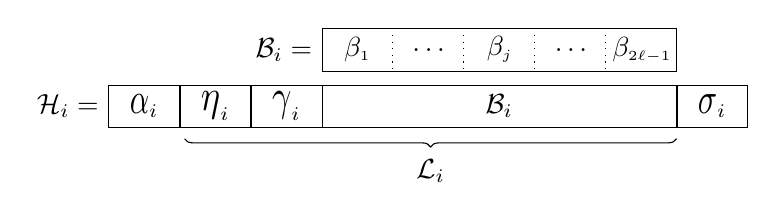
\begin{tikzpicture}

    \node (H) at (0,2) {$\mathcal{H}_i = $};
    \node (alpha) [block=1] at (H.east) {$\ALPHA_{i}$};
    \node (N) [block=1] at (alpha.east) {$\ETA_i$};
    \node (gamma) [block=1] at (N.east) {$\GAMMA_{i}$};
    \node (Bi) [block=5] at (gamma.east) {$\mathcal{B}_i$};
    \node (Sigma) [block=1] at (Bi.east) {$\SIGMA_{i}$};

    \node (B) [block=5, anchor=south west, yshift=5pt] at (Bi.north west)  {};
    \foreach \j in {1,...,4} {
        \draw[dotline] ($(B.north west) + (\j*\width, 0)$) -- ($(B.south west) + (\j*\width, 0)$) {}; 
    }
    \node (beta_1) [blockspace=1] at (B.west)  {$\beta_{\scriptscriptstyle 1}$};
    \node (beta_2) [blockspace=1] at (beta_1.east)  {$\ldots$};
    \node (beta_3) [blockspace=1] at (beta_2.east)  {$\beta_{\scriptscriptstyle j}$};
    \node (beta_4) [blockspace=1] at (beta_3.east)  {$\ldots$};
    \node (beta_5) [blockspace=1] at (beta_4.east)  {$\beta_{\scriptscriptstyle 2\ell-1}$};
    \node[anchor=east] at (B.west) {$\mathcal{B}_i = $};

    % Notes
    \draw [decorate, decoration={brace, amplitude=3pt, mirror, raise=4pt}] (N.215) -- (Bi.south east) node[midway, below=8pt] {$\mathcal{L}_i$};

\end{tikzpicture}}
    \caption{Header structure at hop $i$.}
    \label{fig:header}
\end{figure}

\paragraph{Address representations}
A public directory associates each mixnode identifier $\ETA_i$ with its network address $\mathrm{IP}_i$, allowing address recovery by lookup.
Mixnode address $\mathrm{IP}_i$ is encoded by multiplying $\ZETA_1$ by a publicly computable scalar:
$$ \ETA_i=[h_{\mathbb{F}_q}(\mathrm{IP}_i)]\ZETA_1, \qquad h_{\mathbb{F}_q}:\mathbb{Z}\to\mathbb{F}_q. $$

For destinations, maintaining such a directory would be impractical, and the encoding must not reveal the scalar relating the destination point to $\ZETA_1$.
We therefore use a reversible \emph{try-and-increment} coordinate embedding.
For a destination address $d$, we consider $x_d=d\,2^\kappa+\tau+c$, where $\tau$ is a publicly prescribed $\kappa$-bit padding value (e.g. zeroes or a truncated timestamp).
Starting from zero, the counter $c$ is incremented until a point $(x_d,y_d)\in\mathbb{G}_1$ is found, subject to $\tau+c<2^\kappa$ and $x_d<p$, where $\mathbb{F}_p$ is the curve's coordinate field.
The coordinate $y_d$ is selected using a fixed sign convention.
The padding reserves space for the increment while preserving the address bits. 
The padding and point-selection rules are fixed by the protocol and enforced by the zero-knowledge circuit.
The encoding and decoding functions are thus defined by:
$$ \operatorname{Enc}(d)=(x_d,y_d)=\D{}, \qquad \operatorname{Dec}(\D{}) =\left\lfloor\frac{x_d}{2^\kappa}\right\rfloor. $$ %  \qquad \operatorname{Dec}(\operatorname{Enc}(d)) = d
\todo[inline]{Counter is bounded}

\subsection{Threshold Multi-Authority Setup}
\label{sec:scheme-setup}

Let $\mathcal{A}=\{A_1,\ldots,A_{n_A}\}$ be a set of $n_A$ credential authorities, with issuance threshold $2\leq t\leq n_A$. 
Each authority $A_k$ has a public identifier $x_k\in\mathbb{F}_q$.

At initialization, the authorities are assumed to execute a secure distributed key-generation (DKG) protocol~\cite{DKG}. 
It outputs a Shamir sharing of a secret signing scalar $y$~\cite{ShamirSS}. 
In particular, there exists a polynomial $f\in\mathbb{F}_q[z]$ of degree at most $t-1$ such that:
$$ y=f(0), \qquad y_k=f(x_k),$$
where authority $A_k$ holds only its secret share $y_k$.
The authorities publish the public key $\PSI_1=[y]\ZETA_1$ and the system verification key $\PSI_2=[y]\ZETA_2$ using Lagrange interpolation 
of their shares $[y_k]\ZETA_1$ and $[y_k]\ZETA_2$ from any set $\mathcal{I}$ of at least $t$ authorities, without reconstructing $y$.
$$
\PSI_i = \sum_{k\in\mathcal{I}} [\lambda_k^{\mathcal{I}}]\bigl([y_k]\ZETA_i\bigr) = [y]\ZETA_i, 
\qquad \lambda_k^{\mathcal{I}} = \prod_{\substack{j\in\mathcal{I}\\j\neq k}} \frac{-x_j}{x_k-x_j}.
$$

The system also establishes public parameters $\mathsf{pp}_{\mathrm{zk}}$ for a non-interactive argument of knowledge. 
We instantiate the proof system with Groth16, using a Powers of Tau ceremony followed by a circuit-specific setup to generate the common reference string (CRS) and the associated proving and verification keys. 
Since the authorization circuit is fixed and the blacklist is public, these parameters are generated once and reused across credential requests.


\subsection{Credential Issuance} 
\label{sec:scheme-issuance}
During credential issuance, the authorities require a proof that the requested destination $d$ is not included in the public blacklist $\mathbb{B}$, without learning $d$.
Credential lifetime and subsequent policy changes require a separate validity or revocation mechanism that is outside the scope of this work.

\paragraph{Zero-knowledge Proof}
\label{sec:zk-proof}
The client encode the desired destination $d$ into an elliptic curve point $\D{}=\operatorname{Enc}(d)$, 
samples a fresh blinding scalar $b \in \mathbb{F}_q$, and computes $ \widetilde{\D{}}=[b]\D{}. $
It then generates a NIZK proof $\pi$ for the constraints:
\begin{equation}
    % \label{eq:authorization-relation}
        \begin{aligned}
        &\pi \bigl((\widetilde{\D{}},\mathbb{B});(d,b)\bigr)=1 \quad\Longleftrightarrow\quad
        \begin{cases}
            d\in\{0,\ldots,2^{128}-1\},\\
            d\notin\mathbb{B},\\
            \widetilde{\D{}}
            =[b]\operatorname{Enc}(d).
        \end{cases}
    \end{aligned}
\end{equation}
The public statement consists of the blinded destination $\widetilde{\D{}}$ and the blacklist $\mathbb{B}$.
The destination address $d$ and blinding scalar $b$ form the private witness.
The first condition verify that private destination is in the range of an IP address.
The second condition verify the non-membership to the blacklist.
The last condition binds the non-membership proof to the blinded destination submitted for credential issuance.

\paragraph{Partial Credential Issuance}
\label{sec:scheme-partial-issuance}
The client sends $(\widetilde{\D{}},\pi)$ to at least $t$ authorities.
Each authority verifies the proof $\pi$ using $\mathsf{pp}_{\mathrm{zk}}$ and the provided blinded encoded destination.
A request is rejected if the proof verification fails.
After accepting the request, authority $A_k$ computes $\SIGMA_{k} = [y_k] \widetilde{\D{}}$, and returns the credential share $\SIGMA_{k}$ to the client.


\paragraph{Credential Aggregation}
\label{sec:scheme-aggregation}

After collecting shares from a set $\mathcal{I}$ of at least $t$ distinct authorities, the client aggregates the credential shares using Lagrange interpolation.
It then unblinds the credential by multiplying it by $b^{-1}$. 
This yields the \emph{destination-bound} credential $\SIGMA_{\Delta} = [y] \Delta$.
An honestly generated credential satisfies $e(\SIGMA_{\Delta},\ZETA_2)=e(\Delta,\PSI_2)$.
During issuance, destination blinding and the zero-knowledge proof $\pi$ allow the authorities to verify that the requested destination satisfies the authorization policy without learning the desired destination.




\subsection{Header Construction}
\label{sec:header-construction}

The client selects a route, derives the shared secrets, and constructs the routing layers from the last hop to the first as shown in Figure~\ref{fig:header-construction}.
\begin{figure}
    \centering
    \resizebox{0.6\linewidth}{!}{\centering
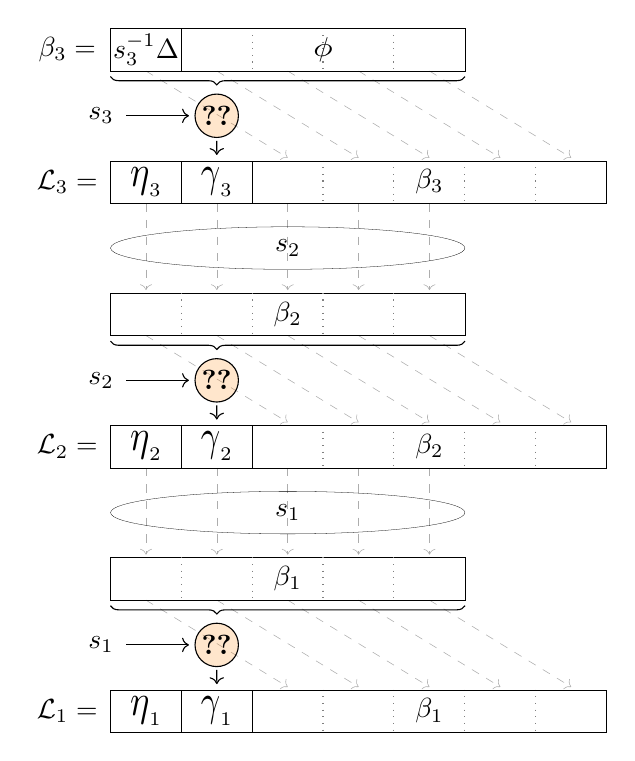
\begin{tikzpicture}
    % \tiny
    \setlength{\y}{0cm}
    \foreach \j in {0,...,4} {
        \node (b3\j) [blockspace=1] at (\j*\width, \y) {};
        \ifnum\j>1  \draw[dotline, gray] (b3\j.north west) -- (b3\j.south west);\fi
    }
    \node (dest) [block=1] at (0, \y) {$s_3^{-1}\Delta$};
    \node (fillers) [block=4] at (\width, \y) {$\PHI$};  
    \node[left of=dest] {$\beta_3 =$};

    % HMAC 3
    \vGap
    \node (hmac3) [eq] at (1.5*\width, \y) {\ref{eq:integrity}};
    \node[left=\width of hmac3] (input_hmac3) {$s_{3}$};
    \vGap
    \node (L3) [blockspace=7] at (0, \y) {};
    \foreach \j in {0,...,6} {\node (L3\j) [blockspace=1] at (\j*\width, \y) {}; }
    \foreach \j in {0,...,4} {
        \node (beta3\j) [blockspace=1] at (2*\width + \j*\width, \y) {}; 
        \ifnum\j>0  \draw[dotline, gray] (beta3\j.north west) -- (beta3\j.south west);\fi
    }
    \node (N3) [block=1] at (0, \y) {$\ETA_{3}$}; 
    \node (gamma3) [block=1] at (\width, \y) {$\GAMMA_3$}; 
    \node (beta3) [block=5] at (2*\width, \y) {$\beta_3$};  
    \node[left of=N3] {$\mathcal{L}_3 =$};

    % ENC 2
    \vGap
    \node [ovale=5] at (0, \y) {$s_2$};
    \vGap
    \node [block=5] at (0, \y) {$\beta_2$};
    \foreach \j in {0,...,4} {
        \node (b2\j) [blockspace=1] at (\j*\width, \y) {}; 
        \ifnum\j>0  \draw[dotline, gray] (b2\j.north west) -- (b2\j.south west);\fi
    }

    % HMAC2
    \vGap
    \node (hmac2) [eq] at (1.5*\width, \y) {\ref{eq:integrity}};
    \node[left=\width of hmac2] (input_hmac2) {$s_{2}$};
    \vGap
    \node (L2) [blockspace=7] at (0, \y) {};
    \foreach \j in {0,...,6} {\node (L2\j) [blockspace=1] at (\j*\width, \y) {}; }
    \foreach \j in {0,...,4} {
        \node (beta2\j) [blockspace=1] at (2*\width + \j*\width, \y) {}; 
        \ifnum\j>0  \draw[dotline, gray] (beta2\j.north west) -- (beta2\j.south west);\fi
    }
    \node (N2) [block=1] at (0, \y) {$\ETA_{2}$}; 
    \node (gamma2) [block=1] at (\width, \y) {$\GAMMA_2$}; 
    \node (beta2) [block=5] at (2*\width, \y) {$\beta_2$};  
    \node[left of=N2] {$\mathcal{L}_2 =$};

    % ENC 1
    \vGap
    \node [ovale=5] at (0, \y) {$s_1$};
    \vGap
    \node [block=5] at (0, \y) {$\beta_1$};
    \foreach \j in {0,...,4} {
        \node (b1\j) [blockspace=1] at (\j*\width, \y) {}; 
        \ifnum\j>0  \draw[dotline, gray] (b1\j.north west) -- (b1\j.south west);\fi
    }

    % HMAC1
    \vGap
    \node (hmac1) [eq] at (1.5*\width, \y) {\ref{eq:integrity}};
    \node[left=\width of hmac1] (input_hmac1) {$s_{1}$};
    \vGap
    \node (L1) [blockspace=7] at (0, \y) {};
    \foreach \j in {0,...,6} {\node (L1\j) [blockspace=1] at (\j*\width, \y) {}; }
    \foreach \j in {0,...,4} {
        \node (beta1\j) [blockspace=1] at (2*\width + \j*\width, \y) {}; 
        \ifnum\j>0  \draw[dotline, gray] (beta1\j.north west) -- (beta1\j.south west);\fi
    }
    \node (N1) [block=1] at (0, \y) {$\ETA_{1}$}; 
    \node (gamma1) [block=1] at (\width, \y) {$\GAMMA_1$}; 
    \node (beta1) [block=5] at (2*\width, \y) {$\beta_1$};  
    \node[left of=N1] {$\mathcal{L}_1 =$};

    %% ARROWS %%
    % hmac 3
    \begin{pgfonlayer}{background}
        \foreach \j in {0,...,4} {
            \draw[->, dashed, very thin, color=unHighlight!80] (b3\j.south) -- ([yshift=+1pt] beta3\j.north);
        }
    \end{pgfonlayer}
    \draw[arrow] (input_hmac3) -- (hmac3.west);
    \draw[arrow] (hmac3.south) -- (gamma3.north);
    \draw [decorate, decoration={brace, amplitude=3pt, mirror, aspect=0.3, raise=2pt}] (dest.south west) -- (fillers.south east);
    % ENC 2
    \begin{pgfonlayer}{background}
        \foreach \j in {0,...,4} {
            \draw[->, dashed, very thin, color=unHighlight!80] (L3\j.south) -- ([yshift=+1pt] b2\j.north);
        }
    \end{pgfonlayer}
    % hmac 2
    \begin{pgfonlayer}{background}
        \foreach \j in {0,...,4} {
            \draw[->, dashed, very thin, color=unHighlight!80] (b2\j.south) -- ([yshift=+1pt] beta2\j.north);
        }
    \end{pgfonlayer}
    \draw[arrow] (input_hmac2) -- (hmac2.west);
    \draw[arrow] (hmac2.south) -- (gamma2.north);
    \draw [decorate, decoration={brace, amplitude=3pt, mirror, aspect=0.3, raise=2pt}] (b20.south west) -- (b24.south east);
    % ENC 1
    \begin{pgfonlayer}{background}
        \foreach \j in {0,...,4} {
            \draw[->, dashed, very thin, color=unHighlight!80] (L2\j.south) -- ([yshift=+1pt] b1\j.north);
        }
    \end{pgfonlayer}
    % hmac 1
    \begin{pgfonlayer}{background}
        \foreach \j in {0,...,4} {
            \draw[->, dashed, very thin, color=unHighlight!80] (b1\j.south) -- ([yshift=+1pt] beta1\j.north);
        }
    \end{pgfonlayer}
    \draw[arrow] (input_hmac1) -- (hmac1.west);
    \draw[arrow] (hmac1.south) -- (gamma1.north);
    \draw [decorate, decoration={brace, amplitude=3pt, mirror, aspect=0.3, raise=2pt}] (b10.south west) -- (b14.south east);

   
\end{tikzpicture}
}
    \caption{DSphinx header construction for a path of length $\ell=3$ (without credential binding). 
    Circled numbers \eq[\color{red}x] refers to Equation x in the paper.}
    \label{fig:header-construction}
\end{figure}


\paragraph{Route and shared secrets}
The client samples an ordered route $(\ETA_1,\ldots,\ETA_\ell)$, a nonce $x_1\in\mathbb{F}_q$, and compute the cryptographic element $\ALPHA_1 = [x_1]\ZETA_1$.
For each hop $i=1,\ldots,\ell$, it uses the mixnode public key $\KAPPA_i=[\mathsf{k}_i]\ZETA_1$ to derive the corresponding shared secrets in cascade as:
\begin{equation}
    % \label{eq:shared_secret}
    \{s_i\}_{i=1}^{\ell} \quad\left\{\quad
    \begin{aligned}
        s_i &= h_{\mathbb{F}_q}\bigl([x_i]\KAPPA_i\bigr),\\
        x_{i+1} &= s_i x_i.
    \end{aligned}
    \right.
\end{equation}

\paragraph{Preprocessing}
The client prepares filler vector $\PHI$ that maintain the routing-layer size during processing. 
Starting with the empty vector $\PHI^{(0)}$, it applies the following recurrence for $i=1,\ldots,\ell-1$, obtaining a filler vector $\PHI^{\ell-1}$ with $2(\ell-1)$ elements in $\mathbb{G}_1$. 
\begin{equation}
    % \label{eq:preprocessing}
    \PHI^{(i)} = [s_i]
    \begin{bmatrix}
        \PHI^{(i-1)}\\
        h_{\mathbb{G}}(s_i)\\
        \ETA_i
    \end{bmatrix}
    \qquad (i=1,\ldots,\ell-1).
\end{equation}

\paragraph{Layer construction.}
The client constructs the routing layers in reverse order, from the last hop $i=\ell$ to the first hop $i=1$.
It initializes the innermost routing vector $\mathcal{B}_\ell$ by concatenating the destination point multiplied by the inverse of the last hop shared secret $[s_\ell^{-1}]\D{}$, with the precomputed filler vector  $\PHI^{\ell-1}$.
\begin{equation}
    % \label{eq:inner_layer}
    \mathcal{B}_\ell = 
    \begin{bmatrix}
        [s_\ell^{-1}]\D{}\\
        \phi^{(\ell-1)}
    \end{bmatrix}
\end{equation}
For each preceding hop $i=\ell-1,\ldots,1$, it forms $\mathcal{B}_i$ by discarding the last two elements of $\mathcal{L}_{i+1}$ and multiplying the resulting vector by $s_i^{-1}$.
For every layer, the client computes an integrity tag $\GAMMA_i$ over $\mathcal{B}_i$ using the shared secret $s_i$, then prepends the hop identifier $\ETA_i$ and the tag to obtain $\mathcal{L}_i$.
\begin{equation}
    \label{eq:layer}
    \mathcal{B}_i = [s_i^{-1}] (\mathcal{L}_{i+1})_{1:2\ell-1},
    \qquad
    \GAMMA_i = \mathsf{HMAC}(s,\mathcal{B}_i),
    \qquad
    \mathcal{L}_i = \begin{bmatrix} \ETA_i \\ \GAMMA_i \\ \mathcal{B}_i \end{bmatrix}.
\end{equation}


\subsection{Credential Binding}
\label{sec:credential-binding}
The client can link the \emph{destination-bound} credential $\SIGMA_{\D{}}$ to the encrypted routing information from the header to obtain a \emph{header-bound} credential $\SIGMA_1$, 
as in eq.~\ref{eq:header_bound_credential}, where $w_i=\prod_{j=1}^{i-1}s_j$, with $w_1=1$, and $IP_i$ is the address of hop $i$.
The client can then send the packet with the following header $\mathcal{H}_1=(\ALPHA_{1},\mathcal{L}_1,\SIGMA_1)$ to the first mixnode.
\begin{equation}
\label{eq:header_bound_credential}
    \SIGMA_{1} = [w_{\ell+1}^{-1}] \SIGMA_{\D{}} + \sum_{i=1}^{\ell}[w_i^{-1} h_{\mathbb{F}_q}\bigl(IP_i\bigr)] \PSI_1,\\
\end{equation}

\subsection{Packet Processing \& Credential Verification}
\label{sec:packet-processing}

Upon receiving header $\mathcal{H}_i=(\ALPHA_i,\mathcal{L}_i,\SIGMA_i)$, mixnode $i$ verifies the credential and the integrity tag before processing and forwarding the header as shown in Figure~\ref{fig:header-processing}.
\begin{figure}
    \centering
    \resizebox{1.\linewidth}{!}{\centering
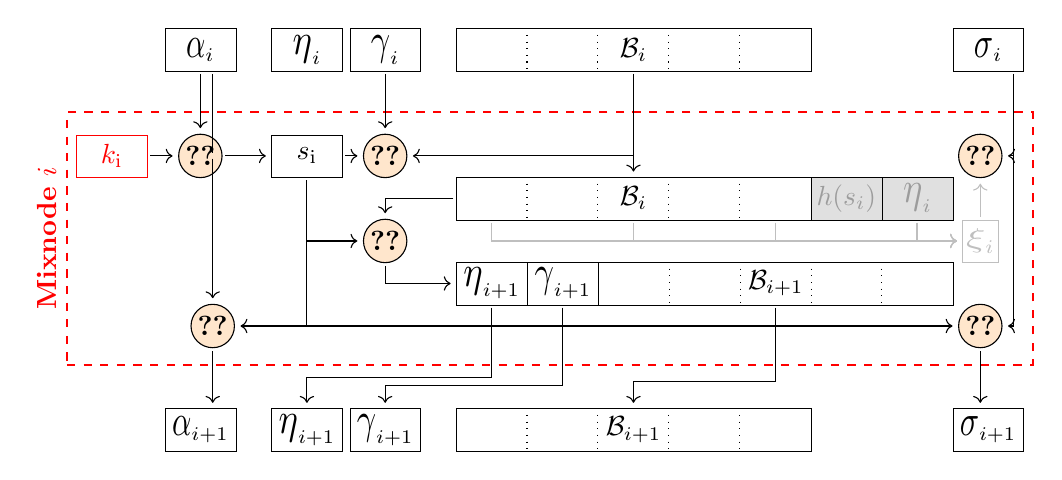
\begin{tikzpicture}
    %% INPUT
    \node (L0) at (0,0) {};
    \node (A) [block=1] at (L0) {$\ALPHA_{i}$};
    \node (N) [block=1] at ($(A.east) + (0.5*\width, 0)$) {$\ETA_i$};
    \node (C) [block=1] at ($(N.east) + (0.1*\width, 0)$) {$\GAMMA_{i}$};
    \node (B) [block=5] at ($(C.east) + (0.5*\width, 0)$)  {$\mathcal{B}_{i}$};
    \node (Sign) [block=1] at ($(B.east) + (2*\width, 0)$) {$\SIGMA_{i}$};

    \foreach \j in {1,...,4} {
        \draw[dotline] ($(B.north west) + (\j*\width, 0)$) -- ($(B.south west) + (\j*\width, 0)$) {}; 
    }

    %% LINE 1 (shared secret, check integrity & decrypt)
    \node (L1) at ($(L0) - (0, 2.5*\height)$) {};
    \node (sk) [block=1, color=red] at ($(L1) - (1.25*\width, 0)$) {\sk{i}};
    \node (ss) [eq] at (A |- L1) {\ref{eq:derive_secret}};
    \node (S) [block=1] at (N.west |- L1)  {\s{i}};
    \node (check) [eq] at (C |- L1)  {\ref{eq:integrity_check}};
    \node (credEq) [eq] at (Sign.-110 |- L1) {\ref{eq:credential_verification}};
 
    %% LINE 2 (decryption up)
    \node (L2) at ($(L1) - (0, 1*\height)$) {};
    \node (BB) [block=5] at (B.west |- L2) {$\mathcal{B}_i$};
    \foreach \j in {1,...,4} {
        \draw[dotline] ($(BB.north west) + (\j*\width, 0)$) -- ($(BB.south west) + (\j*\width, 0)$) {}; 
    }
    \node (pad) [zero_pad=1] at (BB.east) {$h(s_i)$}; 
    \node () [zero_pad=1] at (pad.east) {$\ETA_i$}; 
    \node (xor) [eq] at ($(check |- BB) - (0, 1*\height)$) {\ref{eq:decrypt}};

    %% LINE 3 (decryption down)
    \node (L3) at ($(L2) - (0, 2*\height)$) {};
    \node (N'_) [block=1] at (BB.west |- L3) {$\ETA_{i+1}$};
    \node (C'_) [block=1] at (N'_.east) {$\GAMMA_{i+1}$};
    \node (B'_) [block=5] at (C'_.east) {$\mathcal{B}_{i+1}$};
    \foreach \j in {1,...,4} {
        \draw[dotline] ($(B'_.north west) + (\j*\width, 0)$) -- ($(B'_.south west) + (\j*\width, 0)$) {}; 
    }

    %% LINE 4 (update)
    \node (L4) at ($(L2) - (0, 3*\height)$) {};
    \node (Si) [block=0.5, anchor=center, lightgray] at (credEq |- xor) {$\XI_i$};
    \node (blind) [eq] at (A.-60 |- L4) {\ref{eq:update_alpha}};
    \node (updSign) [eq] at (credEq |- L4) {\ref{eq:update_credential}};
    
    %% BOX
    \node (mixnode) [yshift=1pt, inner ysep=7pt, thick, draw=red, dashed, fit=(sk) (updSign.south-|Sign.east)] {};
    \node[xshift=-7pt, rotate=90] at (mixnode.west) {\color{red} \textbf{Mixnode $i$}};

    %% OUTPUT
    \node (L) at ($(mixnode.south) - (0, 1.5*\height)$) {};
    \node (A') [block=1] at (A.west |- L) {$\ALPHA_{i+1}$};
    \node (N') [block=1] at (N.west |- L) {$\ETA_{i+1}$};
    \node (C') [block=1] at (C.west |- L) {$\GAMMA_{i+1}$};
    \node (B') [block=5] at (B.west |- L)  {$\mathcal{B}_{i+1}$};
    \foreach \j in {1,...,4} {
        \draw[dotline] ($(B'.north west) + (\j*\width, 0)$) -- ($(B'.south west) + (\j*\width, 0)$) {}; 
    }
    \node (Sign') [block=1] at (Sign.west |- L) {$\SIGMA_{i+1}$};
    %% ARROW
    % (4) sum chunks
    \draw[arrow, lightgray] ($(BB.south) + (-2*\width, 0)$) |- (Si);
    \draw[arrow, lightgray] ($(BB.south) + (0*\width, 0)$) |- (Si);
    \draw[arrow, lightgray] ($(BB.south) + (2*\width, 0)$) |- (Si);
    \draw[arrow, lightgray] ($(BB.south) + (4*\width, 0)$) |- (Si);
    % (5) credential verification
    \draw[arrow] (Sign.-40) |- (credEq);
    \draw[arrow, lightgray] (Si) -- (credEq);
    (credEq);
    % (6) shared secret
    \draw[arrow] (A.south -| ss) -- (ss);
    \draw[arrow] (sk) -- (ss);
    \draw[arrow] (ss) -- (S);
    % (7) check
    \draw[arrow] (B.south) |- (check);
    \draw[arrow] (C) -- (check);
    \draw[arrow] (S.east |- check) -- (check); 
    % (8) xor
    \draw[arrow] (B.south) -- (BB.north);
    \draw[arrow] (S.south) |- (xor);
    \draw[arrow] (BB.west) -| (xor);
    \draw[arrow] (xor) |- (N'_.west);
    % (9) blind
    \draw[line] (A.south -| blind) -- (ss -| blind);
    \draw[arrow] (ss -| blind) -- (blind);
    \draw[arrow] (S) |- (blind);
    \draw[arrow] (blind) -- (blind |- A'.north);
    % (10) update credential
    \draw[arrow] (S) |- (updSign);
    \draw[arrow] (Sign.-40) |- (updSign);
    % \draw[arrow, lightgray] (Si.south) -| (updSign);
    \draw[arrow] (updSign.south) -- ($(updSign.south) - (0, 0.9*\height)$) -| (Sign'.110);
    % output
    \draw[arrow] (N'_) -- ($(N'_.south) - (0, 1.7*\height)$) -| (N');
    \draw[arrow] (C'_) -- ($(C'_.south) - (0, 1.9*\height)$) -| (C');
    \draw[arrow] (B'_.south) -- ($(B'_.south) - (0, 1.8*\height)$) -| (B');
\end{tikzpicture}}
    \caption{DSphinx header and its credential processed by mixnode $i$. 
    Circled numbers \eq[\color{red}x] refers to Equation x in the paper.}
    \label{fig:header-processing}
\end{figure}

\paragraph{Credential verification}
The node computes $\XI_i$ by summing the odd-indexed elements of the layer vector $\mathcal{L}_i$, which contains all the route and destination information.
\begin{equation}\label{eq:sum_route}
    \XI_i 
    \;=\; \sum_{j=0}^{\ell}(\mathcal{L}_i)_{2j+1} 
    \;=\; \ETA_i + \sum_{j=1}^{\ell}\BETA_{2j-1}
\end{equation}
It then verifies the pairing equation~\eqref{eq:credential_verification} and discards the packet if the check fails.
Importantly, this verification does not require identifying the vector element containing the destination, preventing the mixnode from determining its position in the route (except at the first and last hops).
\begin{equation}
\label{eq:credential_verification}
    e(\SIGMA_{i}, \ZETA_2)
    \overset{?}{=}
    e(\XI_i, \PSI_2)%,
\end{equation}

\paragraph{Integrity check}
The mixnode derives the shared secret $s_i$ using its secret key $k_i$ with the cryptographic element $\ALPHA_i$ from the header.
Then verify the integrity tag using eq~\eqref{eq:integrity}. 
The packet is discarded if integrity check fails.
\begin{align}
    s_i &=   h_{\mathbb{F}_q}\bigl([k_i]\ALPHA_i \bigr), \label{eq:derive_secret}\\
    \GAMMA_i & \overset{?}{=} \mathsf{HMAC}(s,\mathcal{B}_i). \label{eq:integrity_check}
\end{align}

\paragraph{Layer processing}
After both checks succeed, the next layer $\mathcal{L}_{i+1}$ is processed as in eq.\ref{eq:decrypt}. 
The two firsts elements of $\mathcal{L}_{i+1}$ reveals the next routing identifier $\ETA_{i+1}$ and its integrity tag $\GAMMA_{i+1}$.
While the remaining forms the next encrypted routing information $\mathcal{B}_{i+1}$.
\begin{equation}
    \label{eq:decrypt}
    \mathcal{L}_{i+1} = [s_i] \begin{bmatrix} \mathcal{B}_i \\ h_{\mathbb{G}}(s_i) \\ \ETA_i \end{bmatrix}
\end{equation}

\paragraph{Header update}
The node updates the cryptographic element $\ALPHA$ and credential $\SIGMA$ as in \eqref{eq:update_alpha}  and \eqref{eq:update_credential}.
Since the layer decryption gives $\XI_{i+1}=[s_i]\XI_i$, these updates preserve the pairing equation: 
$ e(\sigma_{i+1},\zeta_2) = e([s_i]\sigma_i,\zeta_2) = e(\xi_i,\psi_2)^{s_i} = e([s_i]\xi_i,\psi_2) = e(\xi_{i+1},\psi_2). $
\begin{equation}
    \label{eq:update_alpha}
    \ALPHA_{i+1} = [s_i]\ALPHA_{i} 
\end{equation}
\begin{equation}
    \label{eq:update_credential}
    \SIGMA_{i+1} = [s_i] \SIGMA_{i} %\bigl( \SIGMA_{i} + \XI_{i} \bigr)
\end{equation}

The mixnode then forwards the updated header $\mathcal H_{i+1}=(\ALPHA_{i+1}, \mathcal{L}_{i+1}, \SIGMA_{i+1})$ to the address associated with $\ETA_{i+1}$. 
At the final hop, $\ETA_{\ell+1}=\D{}$, the destination address $d$ is recovered as $d=\operatorname{Dec}(\D{})$.


% Algorithms
% \begin{figure}
% \centering
% \begin{minipage}{0.47\linewidth}
% \begin{algorithm}[H]
% \small
% \caption{Preprocessing}% (Fig.~\ref{fig:chunk-preprocessing})}
\begin{algorithmic}[1]

\Statex \textbf{Input:}
\Statex \quad
  \begin{tabular}{@{}ll@{}}
    $(s_i)_{i=1}^{\ell}$ & shared secrets \\
    $(N_i)_{i=1}^{\ell}$ & route 
  \end{tabular}
\Statex \textbf{Output:} 
\Statex \quad
  \begin{tabular}{@{}ll@{}}
    $\PHI$ & \hspace{8.5mm} filler chunks \\
  \end{tabular}
\Statex

\State $\PHI \gets \text{empty list}$
\For{$i=1$ \textbf{to} $\ell-1$}
    \State $\PHI \gets
        \PHI \,\Vert\, H_{\mathbb{G}_1}(s_i) \,\Vert\, N_i $
    \State $\PHI \gets [s_i]\PHI$
\EndFor
\State \Return $\PHI$

\end{algorithmic}
% \label{algo:preprocessing}
% \end{algorithm}
% \end{minipage}
% \hfill
% \begin{minipage}{0.47\linewidth}
% \begin{algorithm}[H]
% \small
% \caption{Encryption}
\label{algo:encryption}
\begin{algorithmic}[1]

\Statex \textbf{Input:}
\Statex \quad
  \begin{tabular}{@{}ll@{}}
    $\D{}$                & destination point \\
    $(N_i)_{i=1}^{\ell}$   & route identifiers \\
    $(s_i)_{i=1}^{\ell}$   & shared secrets
  \end{tabular}
\Statex \textbf{Output:}
\Statex \quad
  \begin{tabular}{@{}ll@{}}
    $L_1$ & routing layer
  \end{tabular}
\Statex

\State $\beta_\ell \gets [s_\ell^{-1}]\Delta \,\Vert\, \PHI$
\State $\C{}_\ell \gets \mathsf{HMAC}(s_\ell,\beta_\ell)$
\State $L_\ell \gets (N_\ell, \C{}_\ell, \beta_\ell)$

\For{$i=\ell-1$ \textbf{down to} $1$}
    \State $\beta_i \gets [s_i^{-1}] \: L_{i+1}[1:2\ell-1]$
    \State $\C{i} \gets \mathsf{HMAC}(s_i,\beta_i)$
    \State $L_i \gets (N_i,\C{i}, \beta_i)$
\EndFor

\State \Return $L_1$

\end{algorithmic}
% \label{algo:sttp}
% \end{algorithm}
% \end{minipage}
% \end{figure}
\section{Security}

We consider the security properties introduced by the credential extension and assume the security guarantees of the underlying DSphinx construction established in~\cite{DSphinx}. 
In particular, we focus on the additional security requirements introduced by destination-bound credentials: robustness of the threshold credential system, credential soundness, and preservation of the privacy properties of the underlying packet format.
We assume that the discrete logarithm problem is hard in the underlying elliptic-curve group and that the hash functions used by the construction are modeled as random oracles. 

\subsection{Threshold Authority Security}

Our credential system relies on a threshold set of $A$ authorities, of which at least $t$ are required to issue a valid credential. 
We consider the case of malicious authorities during setup and credential issuance phases. 

\paragraph{Setup Phase}
During setup, the authorities execute a Distributed Key Generation (DKG) protocol based on Shamir secret sharing. 
The resulting signing key $y$ is never reconstructed by any individual authority, and each authority receives only a secret signing share.

The security of this phase requires the underlying DKG to guarantee consistency of the distributed key shares in the presence of malicious participants. 
In particular, a malicious authority must not be able to provide inconsistent shares that cause different honest subsets to derive different signing keys. 
This property is not provided by plain Shamir secret sharing alone and therefore requires a verifiable distributed key-generation protocol, 
for example one based on verifiable secret sharing (VSS)~\cite{VSS, FeldmanVSS, PedersenDKG}.

We consequently assume that the DKG with VSS provides the standard consistency and secrecy guarantees against the considered threshold adversary. 
Under this assumption, any coalition of fewer than $t$ authorities learns no information sufficient to reconstruct the signing key $y$ or to forge credentials.

\paragraph{Credential Issuance}
During normal operation, authorities issue partial credentials on blinded destinations after verifying the authorization proof associated with the request. 
The resulting credential is reconstructed by Lagrange interpolation from at least $t$ valid partial credentials.

Consequently, a malicious authority can prevent or delay credential issuance by refusing to respond or by returning an invalid partial credential, 
but cannot prevent successful issuance as long as the client obtains valid partial credentials from at least $t$ honest authorities. 
More generally, if the client contacts $t+\epsilon$ authorities, credential issuance succeeds in the presence of up to $\epsilon$ non-responsive or malicious authorities, 
provided that at least $t$ contacted authorities return valid partial credentials.

A coalition of $t$ or more authorities is outside this security guarantee: 
such a coalition can reconstruct the distributed signing key and consequently issue arbitrary credentials. 
This is inherent to the threshold trust model rather than a weakness specific to the proposed scheme.


\subsection{Credential Soundness}

We distinguish correctness of honest execution from security against malicious clients. 
An honestly issued credential must remain valid when used in a packet addressed to the destination for which it was issued. 
Conversely, a malicious client should not be able to use credentials issued for other destinations to authorize delivery to an unauthorized destination. 
We first establish correctness and a binding property for the prescribed header construction, then discuss the remaining requirements for credential-forgery resistance.


\paragraph{Correctness}
Let $\Delta$ be the encoded destination of an honestly constructed packet, and let $\SIGMA_{\Delta}=[y]\Delta$ be its destination-bound credential. 
Recall that $w_j=\prod_{k=1}^{j-1}s_k$, with $w_1=1$. Expanding the reverse layer construction gives:
\begin{equation*}
    \XI_1
    = \sum_{j=0}^{\ell}(\mathcal{L}_1)_{2j+1}
    = [w_{\ell+1}^{-1}]\Delta
      + \sum_{j=1}^{\ell}[w_j^{-1}]\ETA_j.
\end{equation*}
Using $\PSI_1=[y]\ZETA_1$ and
$\ETA_j=[h_{\mathbb{F}_q}(IP_j)]\ZETA_1$, the header binding Equation~\eqref{eq:header_bound_credential} yields:
\begin{equation*}
    \begin{aligned}
        \SIGMA_1
        &= [w_{\ell+1}^{-1}]\SIGMA_{\Delta}
           + \sum_{j=1}^{\ell}
             [w_j^{-1}h_{\mathbb{F}_q}(IP_j)]\PSI_1 \\
        &= [y]\left(
             [w_{\ell+1}^{-1}]\Delta
             + \sum_{j=1}^{\ell}[w_j^{-1}]\ETA_j
           \right) \\
        &= [y]\XI_1.
    \end{aligned}
\end{equation*}

This relation is preserved during packet processing. 
At hop $i$, the mixnode removes the first two elements of $\mathcal{L}_i$, appends $h_{\mathbb{G}}(s_i)$ and $\ETA_i$, and multiplies the resulting vector by $s_i$. 
Consequently, the sum of the odd-indexed elements satisfies:
\begin{equation*}
    \XI_{i+1}
    = [s_i]\left(\sum_{j=1}^{\ell}\beta_{2j-1}+\ETA_i\right)
    = [s_i]\XI_i.
\end{equation*}
Since the credential is updated as $\SIGMA_{i+1}=[s_i]\SIGMA_i$, induction gives $\SIGMA_i=[y]\XI_i$ at every hop. 
ilinearity then implies:
\begin{equation*}
    e(\SIGMA_i,\ZETA_2)
    = e([y]\XI_i,\ZETA_2)
    = e(\XI_i,[y]\ZETA_2)
    = e(\XI_i,\PSI_2).
\end{equation*}
Thus, every honest mixnode accepts the credential of an honestly constructed packet.

\paragraph{Credential-Forgery Resistance}
Due to the fixed element in the credential verification equation~\ref{eq:credential_verification},
the credential must satisfy $\SIGMA_i = [y] \XI_i$.
Since the scalar value $x$, such that $\XI_i = x \ZETA_1$, is unknown due to the destination encoding (except if the final destination is a mixnode).
Then the client cannot forge a credential from the public key $\PSI_1$ and must pass by the authorities.

Let's imagine a malicious client want to get credential for an unauthorized destination $\Delta_{\textsf{unauthorized}}$ (i.e. blacklisted destination).
He could request credential for $\Delta_1$ and $\Delta_2$ such that $\Delta_{\textsf{unauthorized}} = \Delta_1 + \Delta_2$.
Then sum the resulting credentials to get a credential for the unauthorized destination:
$$ \SIGMA_{\textsf{unauthorized}} = [y]\Delta_{\textsf{unauthorized}} = [y] \left(\Delta_1 + \Delta_2\right) = [y]\Delta_1 + [y]\Delta_2 = \SIGMA_{\Delta_1} + \SIGMA_{\Delta_2}.$$
However, this attack requires both $\Delta_1$ and $\Delta_2$ to be valid encodings of authorized destinations. 
In particular, their $x$-coordinates must satisfy the prescribed padding constraints. 
Otherwise, verification of the corresponding zero-knowledge proofs would fail, and the authorities would reject the credential requests.

These constraints restrict the points available to the adversary, but do not by themselves establish resistance to this attack. 
A formal security argument requires further analysis of the destination encoding, including the choice of padding parameters.

Alternatively, an adversary could attempt to derive a credential for an unauthorized destination by finding a scalar $x$ such that $\SIGMA_{\textsf{unauthorized}} = [x]\SIGMA_\Delta$.
Since credentials satisfy $\SIGMA_\Delta = [y]\Delta$, this requires $\Delta_{\textsf{unauthorized}} = [x]\Delta$.
Finding such a scalar is an instance of the elliptic-curve discrete logarithm problem.

\subsection{Credential Privacy}

We consider passive observations of honestly generated, authorized packets.
We examine the impact of the credential mechanism on packet unlinkability, client anonymity, destination confidentiality, and its reusability.

\paragraph{Unlinkability}
At each hop, the credential is updated as $\SIGMA_{i+1}=[s_i]\SIGMA_i$, using the same factor as $\ALPHA_{i+1}=[s_i]\ALPHA_i$ in the original Sphinx packet.
All header elements belong to $\mathbb{G}_1$, while credential verification uses the fixed parameters $\ZETA_2$ and $\PSI_2 = [y]\ZETA_2$ in $\mathbb{G}_2$.
In a Type-3 pairing setting, two header components cannot be paired directly, since both belong to $\mathbb{G}_1$.
These observations support the intended unlinkability, but do not by themselves establish that the credential and pairing operation provide no additional linking advantage.

\paragraph{Client Anonymity}
The credential contains no client identifier or client-specific public key.
For a given destination, clients obtain the same unblinded credential $\SIGMA_\Delta=[y]\Delta$, and header binding introduces no client information.
Therefore client anonymity continues to depend on the privacy guarantees of the underlying mixnet, and not the credential.

\paragraph{Destination Confidentiality}
For a destination point $\Delta$, choosing $b$ uniformly from $\mathbb{F}_q$ makes $\widetilde{\Delta}=[b]\Delta$ independent of $\Delta$.
The zero-knowledge proof reveals no additional information beyond the policy outcome.
During forwarding, the destination component in $\mathcal{L}$ and its contribution to $\SIGMA$ are scaled by the inverse product of the remaining hop secrets. 
Destination confidentiality thus relies on these remaining shared secrets, until the final mixnode removes the last factor and recovers the destination.

\paragraph{Reusability}
The destination-bound credential $\SIGMA_\Delta$ is independent of the selected route and can subsequently be bound to any valid route.
The binding in Equation~\eqref{eq:header_bound_credential} depends on the hop secrets, which are derived from the client's fresh random nonce.
Consequently, reusing the same credential along the same route with a fresh nonce rerandomizes the header-bound credential.
This establishes rerandomization under credential reuse.

\appendix

\begin{acks}
The acknowledgments section is defined using the "acks" environment (and NOT an
unnumbered section). This ensures the proper identification of the section in
the article metadata, and the consistent spelling of the heading. Does NOT count
towards page limit. NOT shown (as intended) for anonymous submission. Only edit
for the camera-ready.

Identification of funding sources and other support, and thanks to individuals
and groups that assisted in the research and the preparation of the work should
be included.
\end{acks}

\begin{ethics}
Mandatory section for PoPETs 2027. Does NOT count towards page limit. MUST have
exactly this title and placement (between acknowledgements and references) or
risk desk rejection.

This section should include a justification of the ethics of the work and
information about whether the work was submitted to an external ethics panel
such as an IRB or the Tor Research Safety Board. Research that is deemed to not
have met adequate ethical standards may be rejected on those grounds. Authors
are encouraged to contact PC chairs before submitting to clarify any doubts.
\end{ethics}

\begin{openscience}
Mandatory section for PoPETs 2027. Does NOT count towards page limit. MUST have
exactly this title and placement (between acknowledgements and references) or
risk desk rejection.

To encourage reproducibility, PETS champions open science:
\begin{itemize}
  \item If you provide any research artifacts for the submission, please link
  them here. Make sure that identifying information is removed, perhaps using
  anonymization tools such as \url{https://anonymous.4open.science}.
  \item If you plan to share research artifacts upon acceptance, please briefly
  describe the artifacts here.
  \item If you do not plan to release any research artifacts, please briefly
  justify the decision here.
\end{itemize}

Note that this part is distinct from the artifact review that takes place after
a paper is accepted.
\end{openscience}

\begin{ai}
Mandatory section for PoPETs 2027. Does NOT count towards page limit. MUST have
exactly this title and placement (between acknowledgements and references) or
risk desk rejection.

The goal of this section is to disclose the use of any AI-based tools (e.g.,
ChatGPT, Cursor, Claude Code, FigureLabs) used in the process of producing the
paper. If you have not used any AI-based tools, do not remove this section.
Instead, add a single sentence, ``AI-based tools were not used in this work,''
or similar. 

If you have used AI-based tools to improve writing, please acknowledge it here.
For example, ``The authors used generative AI-based tools to revise the text,
improve flow, and correct any typos, grammatical errors, and awkward phrasing.''
If figures have been significantly or completely generated with AI-based tools,
list the figures here and attribute the AI use in the caption of each figure.

If you used AI-based tools as part of your research methodology, describe it
thoroughly in the text of the paper, and simply acknowledge it here. For
example, "As described in Section 4, AI-based tools were used to assist with
data labeling by generating initial annotations.''

Describe any other AI use here. For example, ``AI-based tools were used to
search for additional related work'', ``AI-based tools were used for
pre-submission review'', or ``AI-based tools were used in the artifact
development and to verify that the methods section of the paper correctly
describes the codebase''. We encourage transparency to help reviewers assess
your work and for fellow scientists to learn about the ethical and constructive
use of AI in the scientific process.

Finally, if you answered yes to any of the cases above or have used AI in any
other way, you are responsible for the accuracy, originality, and integrity of
the output of all AI-based tools. As such, indicate this in this section. For
example, ``We have manually verified and are responsible for the accuracy,
originality, and integrity of the output of all AI-based tools.''
\end{ai}

% The next two lines define the bibliography style to be used (do not change),
% and the bibliography file (use as many or few as you wish).
\bibliographystyle{ACM-Reference-Format}
\bibliography{bib}

% \section{An Appendix Section}
% \label{appendix:first}
% If your work has an appendix, this is the place to put it. Note that in the
% appendix, sections are lettered, not numbered. This document has two appendices,
% Appendix~\ref{appendix:first} and Appendix~\ref{appendix:second}, demonstrating
% the section and subsection identification method.

% \subsection{Part One}

% Lorem ipsum dolor sit amet, consectetur adipiscing elit.

% \subsection{Part Two}

% Etiam commodo feugiat nisl pulvinar pellentesque. Etiam auctor sodales ligula,
% non varius nibh pulvinar semper. Suspendisse nec lectus non ipsum convallis
% congue hendrerit vitae sapien. Donec at laoreet eros.

% \section{Online Resources}
% \label{appendix:second}
% Nam id fermentum dui. Suspendisse sagittis tortor a nulla mollis, in pulvinar ex
% pretium. Sed interdum orci quis metus euismod, et sagittis enim maximus.
% Vestibulum gravida massa ut felis suscipit congue. Nam interdum magna at lectus
% dignissim, ac dignissim lorem rhoncus. Maecenas eu arcu ac neque placerat
% aliquam. Nunc pulvinar massa et mattis lacinia.

\end{document}
\endinput
